\documentclass[10pt,a4paper,titlepage]{article}
\usepackage{amsmath}
\usepackage{amsfonts}
\usepackage{amssymb}
\usepackage[OT1]{fontenc}
\usepackage[utf8]{inputenc}
\usepackage[russian]{babel}
\usepackage{listings}
\usepackage{graphicx}
\usepackage{hyperref}
\hypersetup{
    colorlinks,
    citecolor=black,
    filecolor=black,
    linkcolor=black,
    urlcolor=black
}
\begin{document}
%--titlepage-----
\begin{titlepage}
  \begin{center}
    \large
    \textbf{Федеральное государственное автономное образовательное учреждение\\
    Высшего профессионального образования}

    \vspace{0.25cm}

    Санкт-Петербургский политехнический университет
    \vspace{0.25cm}
    
    Институт компьютерных наук и технологий
    \vspace{0.25cm}
    
    Кафедра компьютерных систем и программных технологий
    \vfill

    \textbf{\textsc{Лабораторная работа №1}}\\[5mm]
    
    {\LARGE Система верстки \TeX{} и расширения \LaTeX}
  \bigskip
    
\end{center}
\vfill

\newlength{\ML}
\settowidth{\ML}{«\underline{\hspace{0.7cm}}» \underline{\hspace{2cm}}}
\hfill\begin{minipage}{0.4\textwidth}
  Выполнил студент\\ группы 53501/3\\
  \underline{\hspace{\ML}} П.\,П.~Жук\\
  «\underline{\hspace{0.7cm}}» \underline{\hspace{2cm}} 2016 г.
\end{minipage}%
\bigskip

\hfill\begin{minipage}{0.4\textwidth}
  Проверил преподаватель\\
  \underline{\hspace{\ML}}\\ К.\,Д.~Вылегжанина\\
  «\underline{\hspace{0.7cm}}» \underline{\hspace{2cm}} 2016 г.
\end{minipage}%
\vfill

\begin{center}
  Санкт-Петербург\\ 2016 г.
\end{center}
\end{titlepage}
%---------------
\tableofcontents
\newpage

\section{Цель работы}
Изучение принципов верстки \TeX, создание первого отчета.

\section{Задание}
\begin{enumerate}
\item Создание минимального файла .tex в простом текстовом редакторе - преамбула, тело документа
\item Компиляция в командной строке - latex, xdvi, pdflatex
\item Оболочка TexMaker, Быстрый старт, Быстрая сборка
\item Создание титульного листа, несколько разделов, списка, несложной формулы
\item Понятие классов документов, подключаемых пакетов
\item Верстка более сложных формул
\end{enumerate}

\section{Ход работы}
Работа проводилась в ОС Windows 8. Предварительно был установлен дистрибутив proTeXt, а также среда Texmaker.
\subsection{Создание минимального файла .tex в простом текстовом редакторе - преамбула, тело документа}
В редакторе <<Блокнот>> был создан простой .tex файл с преамбулой и телом. Соответствующий листинг приведен ниже. Файл называется  1.tex и приложен к отчету.\\
\newline
Листинг 1\\
\fbox{\lstinputlisting{1.tex}}
\subsection{Компиляция в командной строке - latex, xdvi, pdflatex}
Получившийся файл был был скомпилирован в командной строке с помощью latex. В среде Windows утилита xdvi отсутсвует, вместо нее для просмотра .dvi файлов используется yap - yet another previewer. Эта утилита идет в комплекте с дистрибутивом proTeXt. Сконвертировать dvi в pdf с помощью pdflatex мне не удалось из-за непонятной ошибки. Вместо этого я использовал dvipdfm. Ниже показаны результаты работы в командной строке и документ в yap.\\
\newline

\begin{figure}[hbtp]
\centering
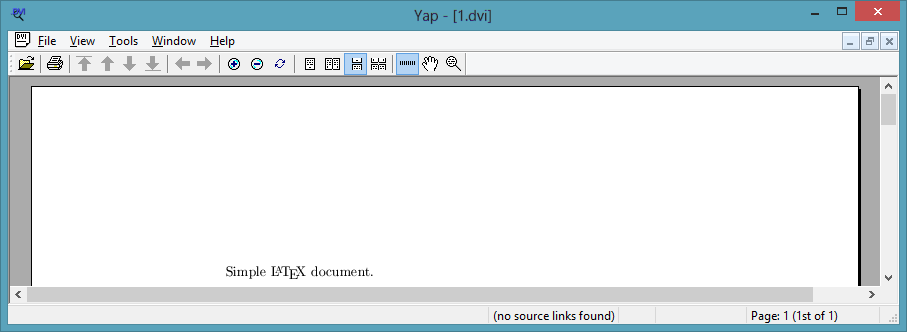
\includegraphics[width=1\linewidth]{yap.png}
\caption{Отображение документа в yap.}
\end{figure}

\begin{figure}[hbtp]
\centering
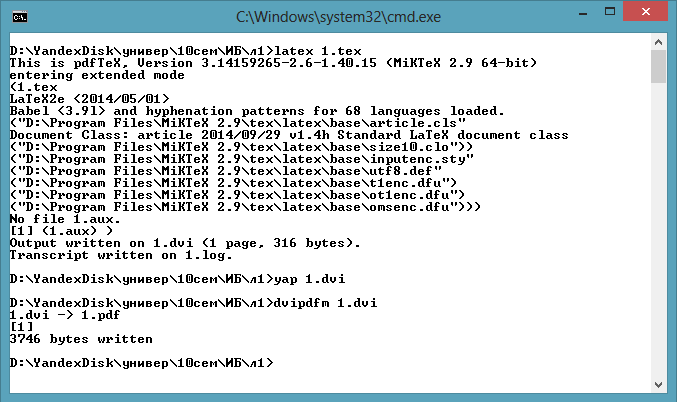
\includegraphics[width=1\linewidth]{CLI.png}
\caption{Результаты работы в командной строке.}
\end{figure}

\subsection{Оболочка TexMaker, Быстрый старт, Быстрая \mbox{сборка}}
TexMaker - удобный редактор документов \LaTeX. Функция <<Быстрый старт>> находится в меню Помощник->Быстрый старт и предоставляет интерфейс для настройки преамбулы документа. Используя быстрый старт, можно настроить класс документа, размер шрифта, указать автора, подключить некоторые из пакетов, и так далее.

\begin{figure}[hbtp]
\centering
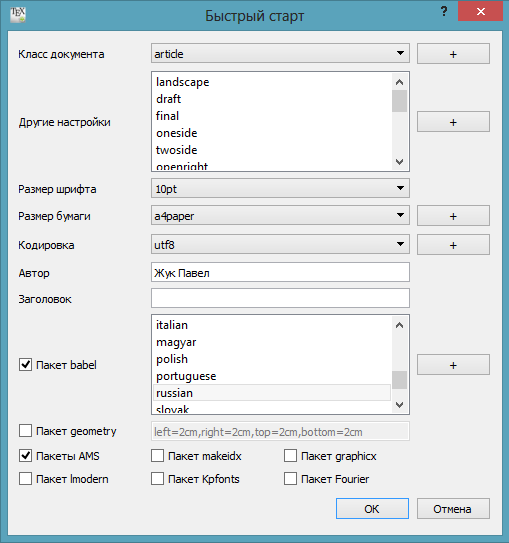
\includegraphics[width=1\linewidth]{FS.png}
\caption{Быстрый старт.}
\end{figure}

Самый простой способ скомпилировать документ является использование команды <<Быстрая сборка>>. В меню Настройка\mbox{->}Настроить Texmaker\mbox{->}Быстрая сборка можно определить последовательность команд, выполняемых при быстрой сборке.

Запустить команду можно кнопкой F1, либо одноименной кнопкой из панели инструментов.

\begin{figure}[hbtp]
\centering
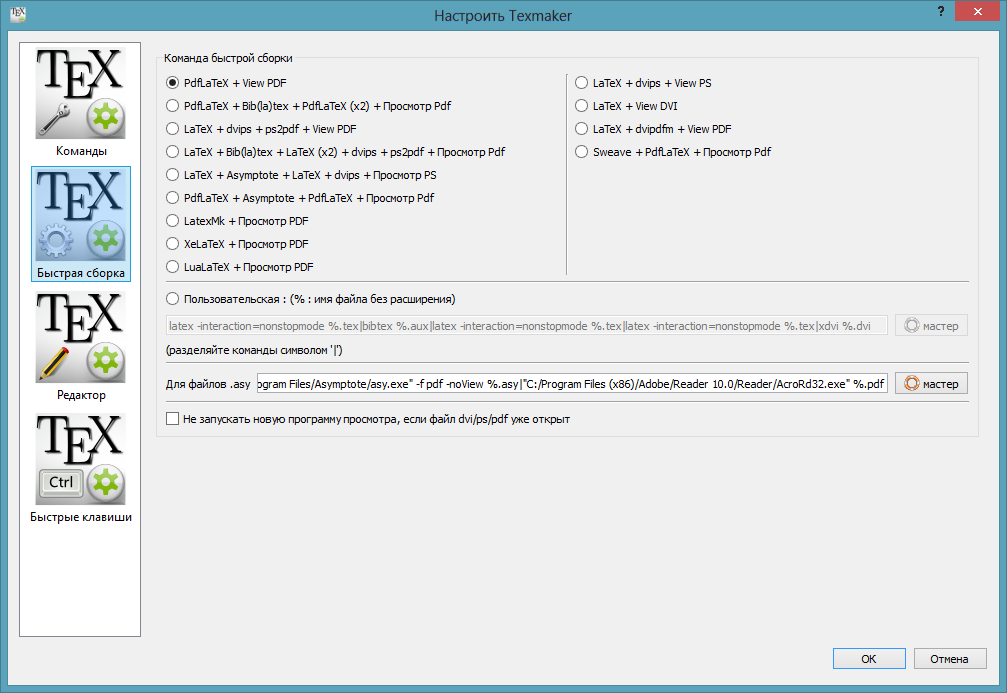
\includegraphics[width=1\linewidth]{QB.png}
\caption{Настройка быстрой сборки.}
\end{figure}

\subsection{Создание титульного листа, несколько разделов, списка, несложной формулы}
Примеры создания титульного листа, нескольких разделов и списка можно посмотреть в исходном файле данного отчета. Пример простой формулы приведен ниже.\\
\begin{equation}
\label{eq:1}
a=\sqrt{b^2 + c^2}
\end{equation}

Соответсвующий данной формуле код:\\
\begin{tabular}{|p{12cm}|}
  \begin{verbatim}
\begin{equation}
\label{eq:2}
a=\sqrt{b^2 + c^2}
\end{equation}
  \end{verbatim}
\end{tabular}\\

Есть возможность ссылаться на определенные ранее формулы. Здесь я обращаюсь к формуле \eqref{eq:1}.
\subsection{Понятие классов документов, подключаемых \mbox{пакетов}}
\textbf{Класс документа} - определяет тип создаваемого документа, что, в свою очередь, задает правила форматирования текста. Он задается командой\\
\begin{tabular}{|p{12cm}|}
  \begin{verbatim}
\documentclass[опции]{класс}
  \end{verbatim}
\end{tabular}\\
\newline
и указывается первым в документе. Класс может быть одним из следующих: \textit{article} - небольшая статья, \textit{report} - более объемный отчет, \textit{book}, \textit{letter}, \textit{beamer} - класс для создания слайдов.

\textit{Опции} - это необязательные параметры, которые изменяют поведение класса, указываются через запятую. Пример:\\
\newline
\begin{tabular}{|p{12cm}|}
  \begin{verbatim}
\documentclass[11pt,twoside,a4paper]{article}
  \end{verbatim}
\end{tabular}\\
\newline
\textbf{Пакеты} - раширения для стандартного \LaTeX. Пакаеты подключаются командой\\
\newline
\begin{tabular}{|p{12cm}|}
  \begin{verbatim}
\usepackage[опции]{пакет}
  \end{verbatim}
\end{tabular}\\
\newline
где \textit{пакет} - имя пакета, а \textit{опции} - список свойств пакета. Некоторые пакеты включены в стандартную поставку \LaTeX, другие приходится устанавливать отдельно.

Пример использования классов и пакетов можно увидеть, например, в .tex файле данного отчета.

\subsection{Верстка более сложных формул}
Ниже приведено несколько примеров более сложных формул.

\begin{equation}
\label{eq:3}
\sum_{\substack{0<i<n \\ 1<j<m}}
P(i,j) =
\sum_{\begin{subarray}{l} i\in I\\
1<j<m
\end{subarray}} Q(i,j)
\end{equation}

\begin{equation}
\label{eq:4}
\mathop{\mathrm{corr}}(X,Y)=
\frac{\displaystyle
\sum_{i=1}^n(x_i-\overline x)
(y_i-\overline y)}
{\displaystyle\biggl[
\sum_{i=1}^n(x_i-\overline x)^2
\sum_{i=1}^n(y_i-\overline y)^2
\biggr]^{1/2}}
\end{equation}

\begin{equation}
\label{eq:5}
\left\{\begin{array}{rcl}y_1&=&a_{11}x_1 + a_{12}x_2 + \ldots + a_{1n}x_n\\
y_2&=&a_{21}x_1 + a_{22}x_2 + \ldots + a_{2n}x_n\\
& \cdots & \\
y_m&=&a_{m1}x_1 + a_{m2}x_2 + \ldots + a_{mn}x_n\\
\end{array}\right.
\end{equation}

\LaTeX{} обладает богатыми возможностями по верстке формул. Для набора формул существуют окружения \textit{math}, \textit{displaymath}, \$\ldots\$, \$\$\ldots\$\$ и некоторые другие. Существует большой набор специальных символов и обозначений. Например: $\prod, \Bigg\}, \mu, \Lambda$ - и многое другое\ldots

\section{Выводы}
К основным преимуществам \LaTeX можно отнести:\\
\begin{itemize}
\item Готовые макеты, задающие стиль документа и позволяющие думать только о его структуре;
\item Удобная верстка математических формул.
\end{itemize}
К минусам можно отести то, что\\
\begin{itemize}
\item Не все возможности \LaTeX{} интуитивно понятны.
\end{itemize}
Впечатления от работы с \LaTeX{ }остались положительными. На данный момент я познакомился с базовыми возможностями. \LaTeX, как инструмент версти текста, обладает большой функциональностью и, как и любой инструмент, требует времени на освоение всех тонкостей и деталей работы с ним.\\
\end{document}